\documentclass{standalone}
\usepackage{tikz}

\begin{document}

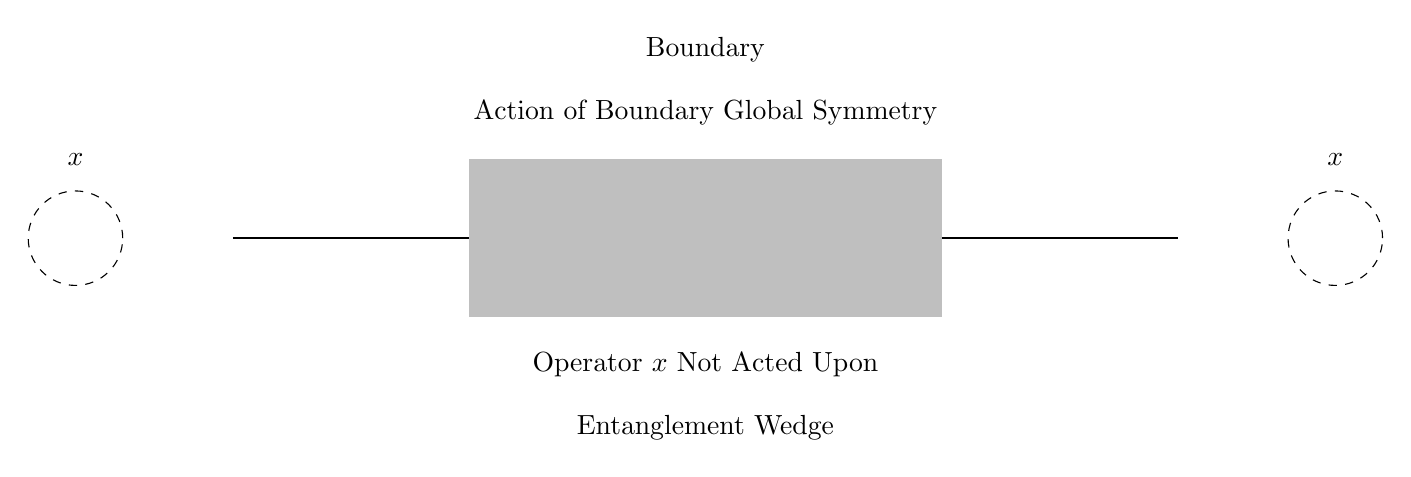
\begin{tikzpicture}[scale=2]
    % Draw the boundary
    \draw[thick] (-3,0) -- (3,0);
    
    % Fill the entanglement wedge with gray color
    \fill[gray!50] (-1.5,-0.5) rectangle (1.5,0.5);
    
    % Label the boundary
    \node at (0,1.2) {Boundary};
    
    % Label the entanglement wedge
    \node at (0,-1.2) {Entanglement Wedge};
    
    % Draw the operator x outside the entanglement wedge
    \draw[dashed] (4,0) circle (0.3);
    \node at (4,0.5) {$x$};
    
    % Draw the operator x inside the entanglement wedge
    \draw[dashed] (-4,0) circle (0.3);
    \node at (-4,0.5) {$x$};
    
    % Label the action of the boundary global symmetry
    \node at (0,0.8) {Action of Boundary Global Symmetry};
    
    % Label the fact that the operator x is not acted upon
    \node at (0,-0.8) {Operator $x$ Not Acted Upon};
\end{tikzpicture}

\end{document}